%\pagestyle{empty}
%\cleardoublepage

\pagestyle{fancy}
\chapter{Referencial Teórico}\label{cap3}

\section{latex}
\label{cap3:latex}

latex é uma linguagem legal...\cite{Adomavicius2005,Stormer2006,Burke2002}


\subsection{Bacana mesmo}%\label{sec:figs}
\label{cap3:bacana}

bacana \ref{cap3:latex}


\section{Outra Seção}
\label{cap3:outra}

Subseção de novo, mas coloco algumas figuras para mostrar resultados (Figura~\ref{fig:last}).
Também é possível definir o tamanho da figura relativamente (e.g., metade da largura do texto; Figura~\ref{fig:last2}).

% Veja a documentação para mais detalhes de como inserir figuras
% O texto entre [] na legenda será utilizado na lista de figuras (no preâmbulo), sendo ideal para substituir legendas maiores
\begin{figure}[htbp]
    \centering
    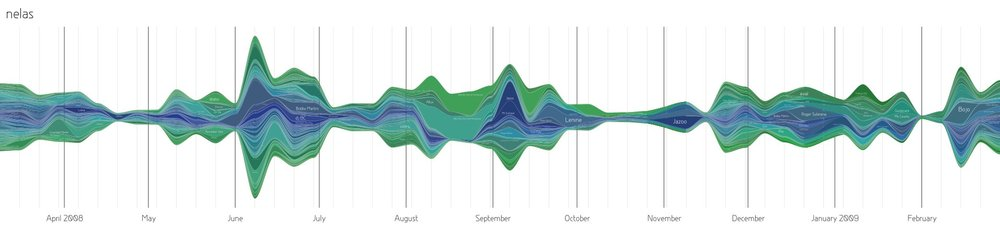
\includegraphics[width=\textwidth]{lastgraph}
    \caption[Figura simples]{Figura abstrata simples com largura igual à largura do texto.}
    \label{fig:last}
\end{figure}

\begin{figure}[htbp]
    \centering
    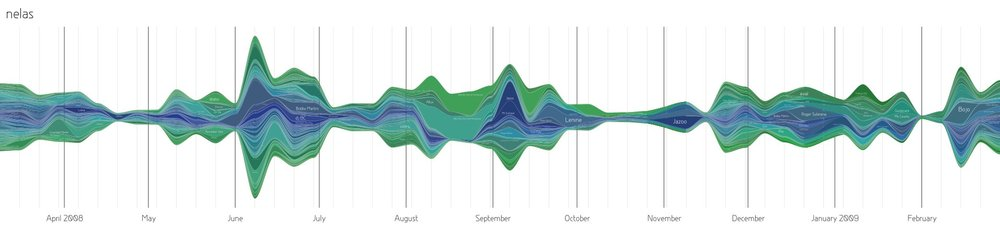
\includegraphics[width=0.5\textwidth]{lastgraph}
    \caption[Outra figura simples]{Figura abstrata simples com largura igual à metade da largura do texto.}
    \label{fig:last2}
\end{figure}

\subsection{Figuras compostas e abreviações}\label{cap2:res:figs2}

Você também pode inserir múltiplas figuras em uma só, permitindo alinhá-las de forma flexível e consistente (ver Figura~\ref{fig:fsm}).

% Usando o pacote nomencl
% Detalhe importante, leia as instruções no site para fazer a lista de abreviações aparecer.
% http://code.google.com/p/mestre-em-latex/wiki/ListaDeAbreviaturas
Para selecionar abreviações que serão incluídas na lista no começo do documento veja o arquivo \texttt{cap2.tex}; como a seguir as células mesenquimais primárias (CMP) iniciam sua ingressão.%
\nomenclature{CMP}{células mesenquimais primárias}

% Note como incluir as sublegendas para cada subfigura (subfloat) e como citá-las na legenda usando o comando subref.
% Note também como incluir as referências às abreviações (nomenclature) utilizadas para que sejam listadas no preâmbulo.
\begin{figure}[htbp]
    \centering
    \subfloat[Subfigura1]{\label{fig:t1}
\includegraphics[width=200pt]{fsm}}\vspace{11pt}
    \subfloat[Subfigura2]{\label{fig:t2}
\includegraphics[width=200pt]{fsm}}\\
    \vspace{-18pt}
    \subfloat[Subfigura3]{\label{fig:t3}
\includegraphics[width=200pt]{fsm}}\vspace{11pt}
    \subfloat[Subfigura4]{\label{fig:t4}
\includegraphics[width=200pt]{fsm}}%
    \caption[Figura com subfiguras]{Exemplo de figura com subfiguras. \subref{fig:t1}~Subfigura1 (\textbf{og}) na lâmina. \subref{fig:t2}~Subfigura2 (\textbf{oppv}). \subref{fig:t3}~Subfigura3 aderida (\textbf{opv}). \subref{fig:t4}~Subfigura4. \textbf{sg}, seio genital; \textbf{ln}, lúmen.}%
    \nomenclature{og}{oogônia}%
    \nomenclature{oppv}{oócitos primários pré-vitelogênicos}%
    \nomenclature{opv}{oócitos primários vitelogênicos}%
    \nomenclature{sg}{seio genital}%
    \nomenclature{ln}{lúmen}
    \label{fig:fsm}
\end{figure}
